\chapter{Scala AST} \label{chapter:scala-ast}

This chapter describes the abstract syntax tree classes that are used in the Scala compiler; the implementations can be found in the \src{scala.reflect.generic.Trees} trait (not to be confused with \src{scala.reflect.Tree}, which provides an undocumented representation of the code at runtime). Note that the list is not complete -- some tree classes are only used during parsing and have already been eliminated at the point tools typically see the code, which is after the typer phase.

We start with the root class \src{Tree}, some of the more interesting traits and abstract classes and then describe the concrete trees. Scala constructs -- syntactic sugar -- that are not represented as trees like parallel assignment and for-comprehensions are described in the last section.

Some remarks on the presentation: on the right of the tree class' name are its ancestor classes and traits. All concrete trees are case classes, so their parameters are listed below the class name. In two-column listings, the one on the left is the original source code and the one on the right is the (cleaned up) result of the \src{Tree}'s \src{toString} method.

\newcommand{\member} [2] {\hfill \begin{footnotesize}\src{#1} \newline \vspace{5pt} \src{#2}\end{footnotesize}\vspace{5pt}}

\section{Base Classes and Traits}

\figref{figure:trees-class-diagram} shows a inheritance diagram of the various tree classes in the compiler.

\begin{figure}
 \centering
 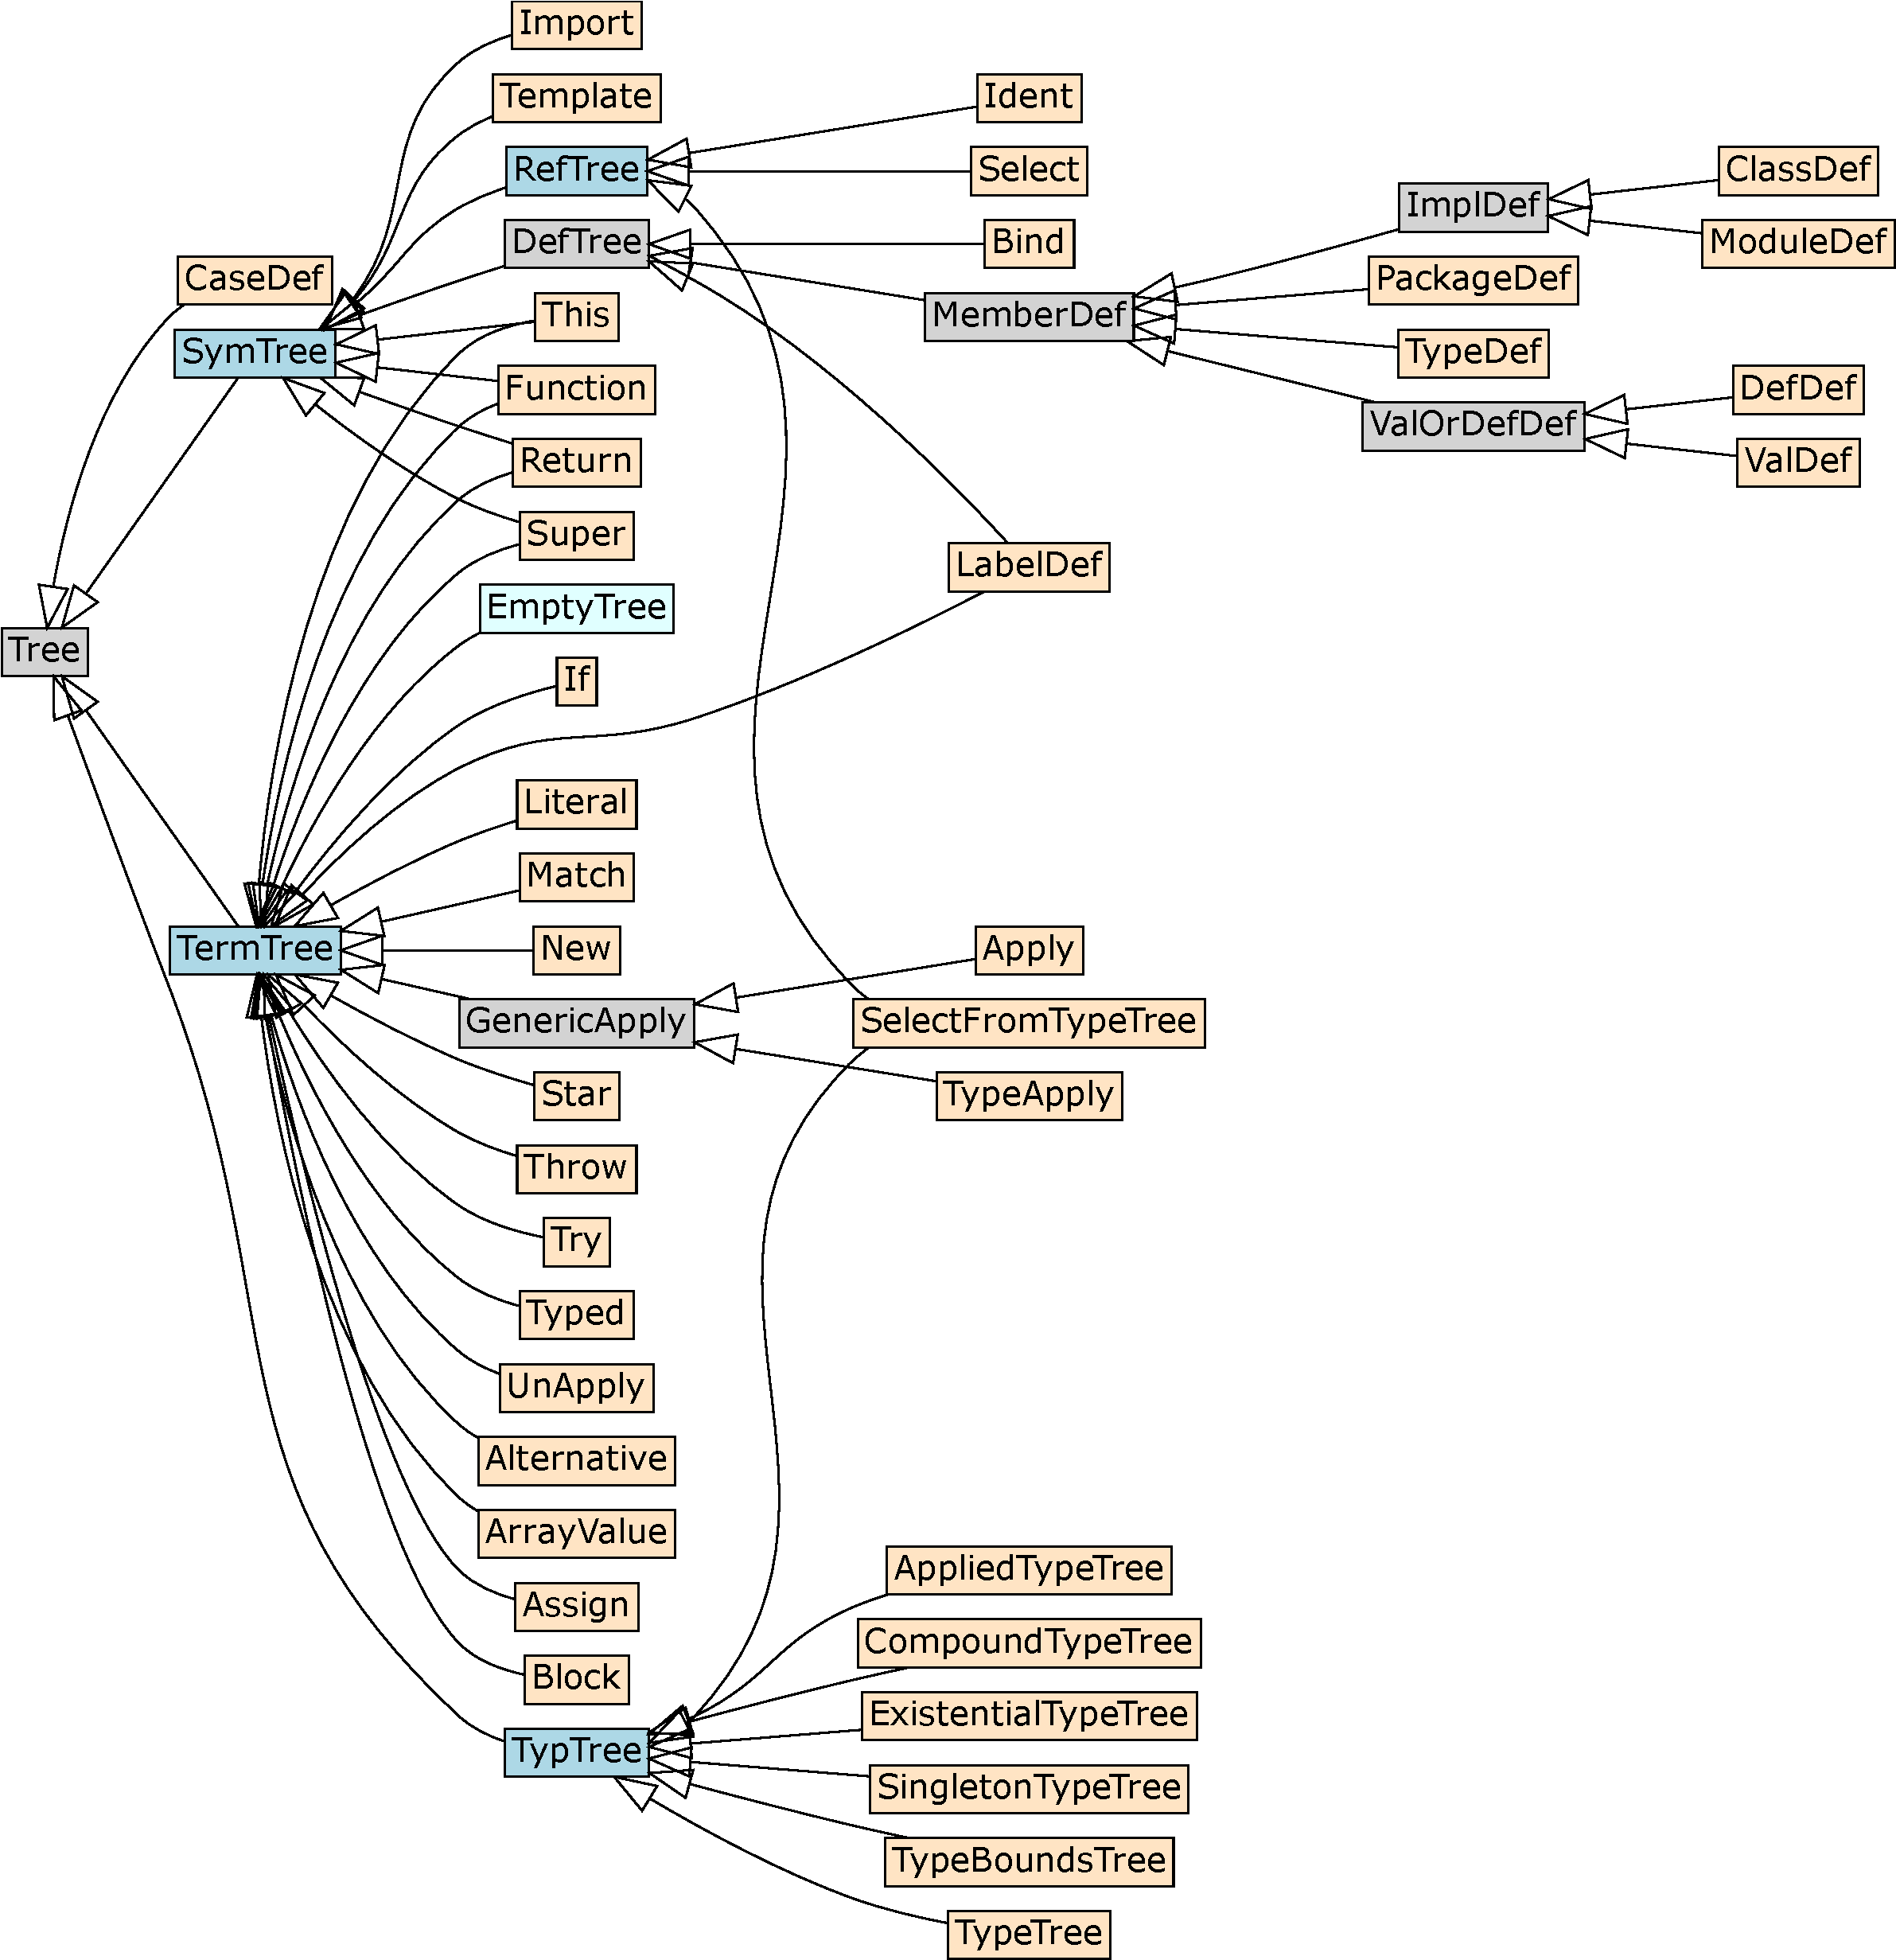
\includegraphics[width=\linewidth]{trees-class-diagram.pdf}
 \caption{The \src{Tree} class with some if its subclasses (some have been omitted for the sake of readability). The gray colored classes are \src{abstract}, blue ones are traits and the bisque colored leafs of the tree are case classes that can be used in pattern matching. The light cyan \src{EmptyTree} is an object (from \cite{ScalaRefactoring}).}
 \label{figure:trees-class-diagram}
\end{figure}

\paragraph{Tree} \hfill \newline

\noindent The \src{Tree} class is the root of all other trees in the AST. It provides some common functionality for all others, for example the position (the \src{\textit{pos}: Position} attribute), the type (\src{\textit{tpe}: Type}), and the symbol (\src{\textit{symbol}: Symbol}). Not all subtrees have symbols or types, so these attributes might return \src{null}.

More operations of the \src{Tree} class are defined in \src{TreeOps}, for example to filter trees or find elements in subtrees.

\paragraph{SymTree} \hfill \begin{footnotesize}\src{Tree}\end{footnotesize} \newline

\noindent The \src{SymTree} trait is extended by all trees that can have a symbol, but it returns \src{NoSymbol} by default.

\paragraph{DefTree} \hfill \begin{footnotesize}\src{SymTree <: Tree}\end{footnotesize} \newline

\noindent The \src{DefTree} class is extended by all trees that define or introduce a new entity into the program. Each \src{DefTree} also has a name and introduces a symbol.

\paragraph{RefTree} \hfill \begin{footnotesize}\src{SymTree <: Tree}\end{footnotesize} \newline

\noindent \src{RefTrees} represent references to \src{DefTrees}. They also have a name and their symbol is the same as their corresponding \src{DefTree's} -- i.e. it can be compared using \src{==}.

\paragraph{Symbol}

Symbols provide another view on the program. Symbols are introduced by \src{DefTrees} and referenced by \src{RefTrees}. Symbols provide a lot more information about the program than the Trees -- there are several dozen \src{isXy} methods defined on symbol to query information. In contrast to Trees, 
Symbols are much more connected to each other: this allows us to resolve class hierarchies or find the enclosing method or class for a symbol. Martin Odersky recorded three videos \cite{ScalaVideos} that walk through the compiler, explaining many Symbol-related concepts.

\paragraph{Position}

\noindent The \src{pos} attribute of the trees is very important for us during refactoring. Unless the compiler runs in IDE mode, it generates \src{OffsetPositions}, which have only a single offset -- the point -- that indicates where a tree comes from; this is sufficient for non-interactive usage. When running in interactive -- IDE -- mode, the compiler generates \src{RangePositions} to represent the source range a tree originally comes from and \src{OffsetPositions} for those trees that were compiler-generated. Ranges have a start-, a point- and an end offset, where the end offset points to the position after the last character.

Range positions satisfy the following invariants, as specified in the \src{Position.scala} source's documentation:

\begin{enumerate}
  \item A tree with an offset position never contains a child with a range position.
  \item If the child of a tree with a range position also has a range position, then the child's range is contained in the parent's range.
  \item Opaque range positions of children of the same node are non-overlapping (this means their overlap is at most a single point).
\end{enumerate}

Due to the first invariant, compiler generated trees with an \src{OffsetPosition} cannot have children with original source code. Sometimes, it is still necessary for the compiler to generate trees that have children with \src{RangePositions}; in these cases, a \src{Transparent} position instead of an \src{OffsetPosition} is used.

There's also a NoPosition object that is assign to trees that have no origin in a source file. In the refactorings, we use this to indicate newly generated trees.

\section{Concrete Trees}

\paragraph{EmptyTree} \hfill \begin{footnotesize}\src{TermTree <: Tree}\end{footnotesize} \newline

\noindent A \src{Tree} object that can stand in for most other trees, it has no position, no type and no symbol. For \src{ValDefs}, the equivalent is the \src{emptyValDef} object.

\paragraph{PackageDef} \member{MemberDef <: DefTree <: SymTree <: Tree}{\textit{pid}: RefTree, \textit{stats}: List[Tree]}

\noindent Describes a package clause with a package identifier and a list of statements. The package identifier is either an instance of \src{Ident} for a package like \src{package a} or an instance of \src{Select} for a package name like \src{package a.b}. The compilation unit root is always a package, even if there is no explicit package declaration present. In this case, the identifier is simply \src{<empty>}. 

According to the Scala Language Specification, the two different notations are equal:

\begin{multicols}{2}
\begin{lstlisting}
package a
package b.c
  
  
\end{lstlisting}

\begin{lstlisting}
package a {
  package b.c {
  }
}
\end{lstlisting}
\end{multicols}

If there exists a top level package definition, its position does not necessarily enclose the whole source file, everything that lies before the \src{package} keyword or after the last statement in the package is not contained in the position. In a package that contains no explicit package declaration and only one statement, the package definition has the same start and end position as the statement, but a different point, which makes them distinguishable.

\paragraph{ClassDef} \member{ImplDef <: MemberDef <: DefTree <: SymTree <: Tree}{\textit{mods}: Modifiers, \textit{name}: Name, \textit{tparams}: List[TypeDef], \textit{impl}: Template}

\noindent The definition for all kinds of classes and traits (objects are defined in \src{ModuleDef}). The definition contains all modifiers, the name and the type parameters. The class' constructor arguments, super classes and its body are all defined in the impl \src{Template}.

Modifiers are a set of \src{abstract, final, sealed, private, protected, trait, case}. Note that the \src{class} keyword is not contained in the modifiers. If the class is anonymous (this can be queried with \src{isAnonymousClass} on the class' symbol), the name is of the form \src{\$anon}.

\paragraph{ModuleDef} \member{ImplDef <: MemberDef <: DefTree <: SymTree <: Tree}{\textit{mods}: Modifiers, \textit{name}: Name, \textit{impl}: Template}

\noindent The definition of a singleton object, similar to the \src{ClassDef} except that a module does not take type parameters. 

\paragraph{Template} \member{SymTree <: Tree}{\textit{parents}: List[Tree], \textit{self}: ValDef, \textit{body}: List[Tree]}

\noindent The implementation of either a \src{ModuleDef} or \src{ClassDef}; also contains early definitions, super types, the self type annotation, and the statements in the class body. In the case of a \src{ClassDef}, it also contains the class' constructor parameters.

The following example illustrates into what constructor parameters and super constructor calls are desugared:

\begin{multicols}{2}
\begin{lstlisting}
class B(i: Int) extends A(i)






\end{lstlisting}
\begin{lstlisting}
class B extends A with ScalaObject {
  <paramaccessor> 
    private[this] val i: Int = _
  def this(i: Int): B = {
    B.super.this(i)
  }
}
\end{lstlisting}
\end{multicols}

To identify the parameters from the list of body statements, we can check the modifiers of all \src{ValDefs} for the \textsc{\src{paramaccessor}} and \textsc{\src{caseaccessor}} flags. In the same way, values and types from the early definition are identified by their \textsc{\src{presuper}} flag. To check whether a value or type belongs to the early definitions, the compiler's \src{treeInfo.isEarlyDef} method can be used.

The super call parameters can be identified as follows: find the constructor \src{DefDef} (\src{symbol.isConstructor} is \src{true}) and then check its body \src{Block} for the following pattern: \src{Apply(Select(Super(\_, \_), \_), args)}. Because only super classes and not traits can have constructor arguments, there can be at most one such super call.

If the self type is not specified, it is the \src{emptyValDef} object. Otherwise, there are several different kinds of self type annotations:

\needspace{11\baselineskip}
\begin{multicols}{2}
\begin{lstlisting}
trait Trait {
}
trait ATrait {
  self =>
}
trait BTrait {
  self: ATrait =>
}
trait CTrait {
  self: BTrait with ATrait =>
}
\end{lstlisting}
\begin{lstlisting}
abstract trait Trait extends scala.AnyRef {
}
abstract trait ATrait extends scala.AnyRef { 
  self: ATrait => 
}
abstract trait BTrait extends scala.AnyRef {
  self: BTrait with ATrait =>
}
abstract trait CTrait extends scala.AnyRef {
  self: CTrait with BTrait with ATrait =>
}
\end{lstlisting}
\end{multicols}

We see that a self type annotation automatically intersects the current trait type with all explicitly named types. Extracting the exact positions of all type names is not trivial and involves searching the value's position for the occurrences of the names.

It is also allowed to use \src{this} for the self type's name. This introduces no alias and the name of the \src{ValDef} is just \src{\_}.

\paragraph{ValDef} \member{ValOrDefDef <: MemberDef <: DefTree <: SymTree <: Tree}{\textit{mods}: Modifiers, \textit{name}: Name, \textit{tpt}: Tree, \textit{rhs}: Tree}

\noindent Value definitions are all definitions of \src{vals}, \src{vars} (identified by the \textsc{\src{mutable}} flag) and parameters (identified by the \textsc{\src{param}} flag).

The modifiers also contain the other properties a value can have: \src{override, abstract, final, implicit, lazy, private, protected}. Whether a modifier is applicable depends on the context where a value is used. A value can also be synthetic, i.e. compiler-generated (identified by the \textsc{\src{synthetic}} flag) -- for example in the following listing of two equivalent statements, a synthetic value is passed to \src{println}:

\begin{lstlisting}
List(1, 2) foreach println
List(1, 2) foreach (println _)
\end{lstlisting}

Even though the value is compiler generated, it sometimes still has a name. In these examples, it is \src{x}, which is the name of \src{println}'s formal parameter. Sometimes, a name of the form \src{x\$1} is used.

Note that not every \src{val} in the source code is necessarily also represented by a \src{ValDef}. The following listing shows how the abstract value in the trait on the left is actually represented by the compiler:

\needspace{3\baselineskip}
\begin{multicols}{2}
\begin{lstlisting}
trait A {
  val a: Int
}
\end{lstlisting}
\begin{lstlisting}
abstract trait A extends scala.AnyRef {
  <stable> <accessor> def a: Int
}
\end{lstlisting}
\end{multicols}

In general, values are always private to the class. For external access, stable accessors are generated, as the following listing illustrates.

\begin{multicols}{2}
\begin{lstlisting}
class A {
  val a = 42

}
\end{lstlisting}
\begin{lstlisting}
class A extends Object with ScalaObject {
  private[this] val a: Int = 42;
  <stable> <accessor> def a: Int = A.this.a
}
\end{lstlisting}
\end{multicols}

Several methods defined on \src{Symbol} can be used to cross-reference between the getters, setters and their underlying value. The \src{accessed} method on a getter or setter symbol returns the underlying value's symbol. To get the corresponding setter or getter from a value, the methods \src{getter} and \src{setter} can be used.

\paragraph{DefDef} \member{ValOrDefDef <: MemberDef <: DefTree <: SymTree <: Tree}{\textit{mods}: Modifiers, \textit{name}: Name, \textit{tparams}: List[TypeDef], \textit{vparamss}: List[List[ValDef]], \textit{tpt}: Tree, \textit{rhs}: Tree}

\noindent The \src{DefDef} trees represent method definitions. Methods can have modifiers that further describe the implementation or constrain its visibility. Every method also has a name, but note that symbolic names are stored in their alphabetic form, to get the original name, the symbol's \src{nameString} method can be used.

In contrast to a \src{ValDef}, a method can be parametrized with types and may have several argument lists. Each argument is represented by a \src{ValDef}.

Abstract methods have the \textsc{\src{deferred}} flag and an \src{EmptyTree} right hand side child.

Finding methods in sub- or super classes requires the use of their \src{symbols}. Super classes can be found via the \src{ancestors} method on the class' symbol. In contrast, moving down the inheritance hierarchy is more expensive. To find all subclasses of a class $C$ one has to collect all other classes in the universe and test each's ancestors for the presence of $C$. Once the class hierarchy is assembled, the definition symbol's \src{overriddenSymbol} method can be used on each class in the hierarchy to gather all overrides.

\paragraph{TypeDef} \member{MemberDef <: DefTree <: SymTree <: Tree}{\textit{mods}: Modifiers, \textit{name}: Name, \textit{tparams}: List[TypeDef], \textit{rhs}: Tree}

\noindent \src{TypeDef} trees are definitions of types. The following listing shows three occurrences -- \src{A, B, C} -- of \src{TypeDefs}:

\begin{lstlisting}
class Types {
  type A = Int
  type B >: Nothing <: AnyRef
  def d[C] ...
}
\end{lstlisting}

Just as the other member definitions trees (\src{ValDef} and \src{DefDef}), type definitions can have modifiers.

\paragraph{LabelDef} \member{DefTree <: SymTree  <: Tree $\wedge$ TermTree <: Tree}{name: Name, params: List[Ident], rhs: Tree}

\noindent The \src{LabelDef} tree is used to represent \src{while} and \src{do \ldots while} loops. The name holds the name of the label.

The Scala language specification \cite{ScalaLanguageSpecification} says 

\begin{quotation}
The while loop expression \src{while ($e_1$) $e_2$} is typed and evaluated as if it was an application of \src{whileLoop ($e_1$) ($e_2$)} where the hypothetical function \src{whileLoop} is defined as follows.

\begin{lstlisting}
def whileLoop(cond: => Boolean)(body: => Unit): Unit =
if (cond) { body ; whileLoop(cond)(body) } else {}
\end{lstlisting}

\end{quotation} 

We can also see this when we print the \src{LabelDef}:

\begin{multicols}{2}
\begin{lstlisting}
while (true != false) println("loop")





while(true) {
  println("loop")
  println("loop")
}






\end{lstlisting}
\begin{lstlisting}
while$1(){
  if (true != false) {
      println("loop")
      while$1()
    }
}
while$2(){
  if (true)
    {
      {
	println("loop");
	println("loop")
      }
      while$2()
    }
}
\end{lstlisting}
\end{multicols}

We can see that multiple statements in the body create an additional block that wraps the statements. The \src{do \ldots while} loops are represented in a similar way:

\begin{multicols}{2}
\begin{lstlisting}
do println("loop") while (true)




\end{lstlisting}
\begin{lstlisting}
doWhile$1(){
  println("loop")
  if (true)
    doWhile$1()
}
\end{lstlisting}
\end{multicols}

Thanks to pattern matching, extracting the relevant parts is easy:

\begin{lstlisting}
case LabelDef(_, _, If(cond, body, _)) // while with single expression
case LabelDef(_, _, If(cond, Block((body: Block) :: Nil, _) // while
case LabelDef(_, _, Block(body, If(cond, _, _))) // do While
\end{lstlisting}

\paragraph{Import} \member{SymTree <: Tree}{\textit{expr}: Tree, \textit{selectors}: List[ImportSelector]}

\noindent An import statement imports one or many names -- the selectors -- from a package or object \src{expr}. An \src{ImportSelector} has two name-position pairs, the first one stands for the imported name and the second one is an optional renaming. Wildcard imports are also represented with an \src{ImportSelector}.

Import trees can also be comma separated, in this case, only the first import includes the \src{import} keyword in its position.

\paragraph{Block} \member{TermTree <: Tree}{\textit{stats}: List[Tree], \textit{expr}: Tree}

\noindent A \src{Block} encloses a list of statements in \src{\{ \ldots \}} and returns the value of its \src{expr} child. \src{Block} trees are only generated when needed -- for example, the right hand side of a \src{DefDef} with a single expression is not a \src{Block} but the expression itself, even when the expression is enclosed in \src{\{ \ldots \}}.

The \src{expr} is usually the last line of a block, with regards to their positions, but this is not always the case. For example, when creating an anonymous class, the class is introduced with a compiler generated name and then instantiated:

\needspace{6\baselineskip}
\begin{multicols}{2}
\begin{lstlisting}
val a = new {
}




\end{lstlisting}
\begin{lstlisting}
val a: java.lang.Object = {
  final class $anon extends scala.AnyRef {
    %\ldots%
  }
  new $anon()
}
\end{lstlisting}
\end{multicols}

\paragraph{CaseDef} \member{Tree}{\textit{pat}: Tree, \textit{guard}: Tree, \textit{body}: Tree}

\noindent The body of a \src{Match} tree contains a number of \src{CaseDefs} trees. The guard can be an empty tree if it is not present. Note that even though the \src{if} keyword is used, the tree is not an \src{If} tree.

Patterns can be of different form, the catch-all \src{\_} is simply an \src{Ident} tree, whereas extractors are represented through the \src{UnApply} trees. Patterns that use an \src{@} binding or are restricted by type with \src{:} are \src{Bind} trees. The body can again be an arbitrary tree.

\paragraph{Alternative} \member{TermTree <: Tree}{\textit{trees}: List[Tree]}

\noindent \src{Alternative} trees are used in case definitions to match on alternative clauses, they are separated by \src{|}.

\paragraph{Star} \member{TermTree <: Tree}{\textit{elem}: Tree}

\noindent Patterns can choose to match the whole remainder of an extracted sequence using the \src{\_*} pattern, as in the following example:

\begin{lstlisting}
"abcde".toList match {
  case Seq(car, cadr, _*) => car 
}
\end{lstlisting}

The wildcard-star is represented by the \src{Star} tree.

\paragraph{Bind} \member{DefTree <: SymTree <: Tree}{\textit{name}: Name, \textit{body}: Tree}

\noindent The \src{Bind} tree binds a name to an expression and is used in the patterns of \src{CaseDef}. We can see from some examples that several seemingly different syntax variations are all represented in a uniform way in the AST:

\begin{multicols}{2}
\begin{lstlisting}
list match {
  case i => %\ldots%
  case i: Int => %\ldots%
  case a @ i: Int => %\ldots%
}
\end{lstlisting}
\begin{lstlisting}
list match {
  case (i @ _) => %\ldots%
  case (i @ (_: Int)) => %\ldots%
  case (a @ (i @ (_: Int))) => %\ldots% 
}
\end{lstlisting}
\end{multicols}

\paragraph{UnApply} \member{TermTree <: Tree}{\textit{fun}: Tree, \textit{args}: List[Tree]}

\noindent When an extractor object is used in the pattern of a case definition, an \src{UnApply} tree is used. The arguments of \src{UnApply} can then be more  patterns.

\begin{multicols}{2}
\begin{lstlisting}
case Ex(i) => i

case a @ Ex(i) => i

case a @ Ex(i: Int) => i

\end{lstlisting}
\begin{lstlisting}
case Ex.unapply(<unapply-selector>) 
  <unapply> ((i @ _)) => i
case (a @ Ex.unapply(<unapply-selector>) 
  <unapply> ((i @ _))) => i
case (a @ Ex.unapply(<unapply-selector>) 
  <unapply> ((i @ (_: Int)))) => i
\end{lstlisting}
\end{multicols}

\paragraph{Function} \member{TermTree <: Tree $\wedge$ SymTree <: Tree}{vparams: List[ValDef], body: Tree}

\noindent The \src{Function} tree contains a single list of parameters and a body for the implementation. The following listing shows various usages of the \src{Function} tree and how their trees look like.

\begin{multicols}{2}
\begin{lstlisting}
list foreach println


list foreach (println _)


list foreach (i => println(i))
list foreach ((i: Int) => println(i))
list foreach {
  case i => println(i)
}
\end{lstlisting}
\begin{lstlisting}
list foreach ({
  ((x: Any) => println(x))
})
list foreach ({
  ((x: Any) => println(x))
})
list foreach (((i: Int) => println(i)))
list foreach (((i: Int) => println(i)))
list foreach (((x0$1: Int) => x0$1 match {
  case (i @ _) => println(i)
}))
\end{lstlisting}
\end{multicols}

In the first two examples, the functions are encapsulated in an additional \src{Block} -- hence the curly braces. When the function parameter does not have a name, the compiler generates one and marks it with the \textsc{\src{synthetic}} flag. In the last example, we see that the pattern matching on the parameter is made explicit in the AST.

\paragraph{Assign} \member{TermTree <: Tree}{\textit{lhs}: Tree, \textit{rhs}: Tree}

\noindent \src{Assign} trees are not used for all \src{=} calls, only for non-initial assignments to variables. Calls to setter methods are not represented by \src{Assign} trees but are regular method calls.

\paragraph{If} \member{TermTree <: Tree}{\textit{cond}: Tree, \textit{thenp}: Tree, \textit{elsep}: Tree}

\noindent An \src{If} expression consists of three parts: the condition, the then part and the else part. If the else part is omitted, the literal \src{()} of type \src{Unit} is generated and the type of the conditional is set to an upper bound of \src{Unit} and the type of the then expression, usually \src{Any}.

\src{else if} terms are implemented using nested if conditionals. We can see this in the following listing.

\begin{multicols}{2}
\begin{lstlisting}
if (a)
  b
else if (c)
  d
else
  e

\end{lstlisting}
\begin{lstlisting}
if (a)
  b
else
  if (c)
    d
  else
    e
\end{lstlisting}
\end{multicols}

Note that the \src{if} used in pattern matching guards is not an \src{If} tree but a designated member of the \src{CaseDef} tree.

\paragraph{Match} \member{TermTree <: Tree}{\textit{selector}: Tree, \textit{cases}: List[CaseDef]}

\noindent A match tree is used to represent a pattern match, with the \src{selector} being the tree that is matched against. When a pattern matching expression is used as the body of a function, the selector is a synthetic value:

\begin{multicols}{2}
\begin{lstlisting}
list foreach {
  case i => println(i)
}
\end{lstlisting}
\begin{lstlisting}
list foreach (((x0$1: Int) => x0$1 match {
  case (i @ _) => println(i)
}))
\end{lstlisting}
\end{multicols}

\paragraph{Return} \member{TermTree <: Tree $\wedge$ SymTree <: Tree}{\textit{expr}: Tree}

\noindent The \src{Return} tree contains an expression that constitutes the return value. For \src{return} statements without an expression, the compiler generates a \src{()} literal.

\paragraph{Try} \member{TermTree <: Tree}{\textit{block}: Tree, \textit{catches}: List[CaseDef], \textit{finalizer}: Tree}

\noindent The \src{Try} tree represents \src{try \ldots catch} expressions. Both the catches and the finalizer are optional.

\paragraph{Throw} \member{TermTree <: Tree}{\textit{expr}: Tree}

\noindent The \src{Throw} tree stands for the \src{throw} keyword and its expression.

\paragraph{New} \member{TermTree <: Tree}{\textit{tpt}: Tree}

\noindent The \src{New} tree represents \src{new} statements, the \src{tpt} member is the type that is being instantiated.

\paragraph{Typed} \member{TermTree <: Tree}{\textit{expr}: Tree, \textit{tpt}: Tree}

\noindent The \src{Typed} tree is used whenever an expression is annotated with a type. For example, in the following listing, the second and third occurrences of \src{Int} are \src{Typed} trees:

\begin{lstlisting}
val a: Int = 42: Int
println(a: Int)
\end{lstlisting}

\src{Typed} trees are also used in pattern matching when the match checks the type of the underlying object.

\paragraph{TypeApply} \member{GenericApply <: TermTree <: Tree}{\textit{fun}: Tree, \textit{args}: List[Tree]}

\noindent \src{TypeApply} trees are used whenever a type is applied to a generic method. For example, in the following listing, both expressions on the left are represented by the same AST on the right.

\begin{multicols}{2}
\begin{lstlisting}
List(1,2,3)

List[Int](1,2,3)


\end{lstlisting}
\begin{lstlisting}
Apply(
  TypeApply(
    Select(%\ldots%, "apply"), 
    List(Int)), 
  List(1,2,3))
\end{lstlisting}
\end{multicols}

\paragraph{Apply} \member{GenericApply <: TermTree <: Tree}{\textit{fun}: Tree, \textit{args}: List[Tree]}

\noindent Function application is represented with \src{Apply} trees. The \src{fun} is often a \src{Select} tree that specifies the function name and \src{args} are the actual parameters.

\paragraph{Super} \member{TermTree <: Tree $\wedge$ SymTree <: Tree}{\textit{qual}: Name, \textit{mix}: Name}

\noindent The \src{Super} tree represents a \src{super} call, with optional qualifier and super class specifier:

\begin{lstlisting}
trait A {
  def x = 42
}
trait B extends A {
  override def x = 43
}
class C extends A with B {
  println(super[A].x)
}
\end{lstlisting}

\paragraph{This} \member{TermTree <: Tree $\wedge$ SymTree <: Tree}{\textit{qual}: Name}

\noindent The \src{This} tree represents the \src{this} reference, with an optional qualifier:
\needspace{5\baselineskip}
\begin{lstlisting}
class Outer {
  class Inner {
    val outer = Outer.this
  }
}
\end{lstlisting}

\paragraph{Select} \member{RefTree <: Symtree <: Tree}{\textit{qualifier}: Tree, \textit{name}: Name}

\noindent The \src{Select} tree occurs on places that select a name from a qualifier, e.g. in method calls. Note that the typer fully qualifies references as illustrated in the following listing.

\begin{multicols}{2}
\begin{lstlisting}
class A {
  val a = %\ldots%
  val b = a
}
\end{lstlisting}
\begin{lstlisting}  
class A {
  val a = %\ldots%
  val b = A.this.a
}
\end{lstlisting}
\end{multicols}

As usual, these generated trees then have an \src{OffsetPosition}.

\paragraph{Ident} \member{RefTree <: Symtree <: Tree}{\textit{name}: Name}

\noindent Holds a \src{Name}, which can be generated (check with \src{symbol.isSynthetic}) by the compiler. Note that the name is in its alphabetic form; the real name can be found via the tree's symbol.

\paragraph{Literal} \member{TermTree <: Tree}{value: Constant}

\noindent All literals are represented by \src{Literal} trees. All possible kinds of constants are listed in the \src{Constant} trait.

\paragraph{TypeTree} \member{AbsTypeTree <: TypTree <: Tree}{\textit{original}: Tree}

\noindent From the Scala compiler's documentation \cite{AbsTypeTree}: 

\begin{quote}
A synthetic term holding an arbitrary type. Not to be confused with with TypTree, the trait for trees that are only used for type trees. TypeTrees are inserted in several places, but most notably in \src{RefCheck}, where the arbitrary type trees are all replaced by TypeTrees.\end{quote}

The original type tree is still accessible via the \src{TypeTree}'s \src{original} member. Note that the standard tree \src{Traverser} and \src{Transformer} visitors do not traverse into the \src{original} subtree.

\paragraph{SingletonTypeTree} \member{TypTree <: Tree}{\textit{ref}: Tree}

\noindent Whenever the \src{.type} expression is used, the tree is represented by a \src{SingletonTypeTree} tree. 

\paragraph{SelectFromTypeTree} \member{TypTree <: Tree $\wedge$ RefTree <: SymTree <: Tree}{\textit{qualifier}: Tree, \textit{name}: Name}

\noindent Type selection of the form \src{qualifier\#name} is represented with the \src{SelectFromTypeTree} tree.

\paragraph{CompoundTypeTree} \member{TypTree <: Tree}{\textit{templ}: Template}

\noindent An intersection type is represented by a \src{CompoundTypeTree}. Note that the tree contains a \src{Template}, this is because the compound type can have an optional refinement: 

\begin{lstlisting}
trait A
trait B
%\ldots% A with B {
  %\ldots%
}
\end{lstlisting}

\paragraph{AppliedTypeTree} \member{TypTree <: Tree}{\textit{tpt}: Tree, \textit{args}: List[Tree]}

\noindent When a type is applied to a polymorphic function, a \src{TypeApply} tree is used. When a type is applied to an other type, an \src{AppliedTypeTree} is used.

\paragraph{TypeBoundsTree} \member{TypTree <: Tree}{\textit{lo}: Tree, \textit{hi}: Tree}

\noindent Whenever a type is constrained to lower or upper bounds, \src{TypeBoundsTree} represents these bounds. If one of the bounds is omitted, the compiler inserts \src{Nothing} respectively \src{Any} for the missing lower or upper bound. This is illustrated in the following example:

\begin{multicols}{2}
\begin{lstlisting}
type B >: Nothing <: AnyRef
type C >: String
type D <: AnyRef
\end{lstlisting}
\begin{lstlisting}  
type B >: Nothing <: AnyRef
type C >: String <: Any
type D >: Nothing <: AnyRef
\end{lstlisting}
\end{multicols}

\paragraph{ExistentialTypeTree} \member{TypTree <: Tree}{\textit{tpt}: Tree, \textit{whereClauses}: List[Tree]}

\noindent Existential types are represented with a \src{ExistentialTypeTree}. In Scala, there exist two notations for existentials:

\begin{lstlisting}
List[_]
List[T] forSome { type T }
\end{lstlisting}

Both are represented the same way in the AST, with their full notation:

\begin{lstlisting}
List[_$1] forSome { 
  <synthetic> type _$1 >: _root_.scala.Nothing <: _root_.scala.Any
}
List[T] forSome { 
  type T >: _root_.scala.Nothing <: _root_.scala.Any
}
\end{lstlisting}

Note that the existential type tree is stored in another \src{TypeTree}'s \src{orig} member, which is not traversed and transformed by the Scala compiler's \src{Traverser} and \src{Transformer} classes.

\section{Other AST Constructs} \label{section:other-ast-constructs}

\subsubsection*{For Comprehensions}

\noindent \src{For} or sequence comprehensions are a purely syntactic construct; in the AST, they are represented with \src{foreach}, \src{withFilter}, \src{map}, and \src{flatMap} calls. The following listing shows some examples. 

\needspace{10\baselineskip}
\begin{lstlisting}
val xs = 1 to 10 toList
val ys = 1 to 10 toList

val coordinates1: List[(Int, Int)] = for(x %$\leftarrow$% xs; y %$\leftarrow$% ys) yield (x %$\rightarrow$% y)
// is equal to
val coordinates2: List[(Int, Int)] = xs.flatMap(x %$\Rightarrow$% ys.map(y %$\Rightarrow$% (x %$\rightarrow$% y)))

for(x %$\leftarrow$% xs if x %\%% 2 == 0) println(x)
// is equal to
xs.withFilter(x %$\Rightarrow$% x %\%% 2 == 0).foreach(x %$\Rightarrow$% println(x))
\end{lstlisting}


\subsubsection*{Multiple Assignment}

\noindent Scala's multiple or parallel assignment syntax is just an abbreviation for a more complex pattern match expression. The following listing shows the desugared form for the call \src{val (a, b) = getPair()}:

\begin{lstlisting}
def getPair() = (1, 2)

val x$1 = getPair() match {
  case (a, b) %$\Rightarrow$% (a, b)
}

val a = x$1._1
val b = x$1._2
\end{lstlisting}

The same transformation is also performed when extractors are involved in the assignment:

\begin{lstlisting}
val MyRegex = """(\w)(.*)""".r
val MyRegex(firstGroup, secondGroup) = "Hello"
\end{lstlisting}

becomes:

\begin{lstlisting}
val MyRegex = """(\w)(.*)""".r
val x$1 = "Hello" match {
  case MyRegex(firstGroup, secondGroup) %$\Rightarrow$% (firstGroup, secondGroup)
}

val firstGroup = x$1._1
val secondGroup = x$1._2
\end{lstlisting}

\subsubsection*{Named Arguments}

Named arguments are desugared into a series of local values that are then passed in the right order to the method. That is, the following code:

\begin{lstlisting}
def p(first: String, second: Int) = ()

p(second = 42, first = "-")      
\end{lstlisting}

is represented as:

\begin{lstlisting}
def p(first: String, second: Int): Unit = ()
{
  val x$1 = 42
  val x$2 = "-"
  Account.this.p(x$2, x$1)
}
\end{lstlisting}

This is described in the first Scala Improvement Document \cite{SID1}.



